\documentclass{standalone}
\usepackage{tikz}
\usetikzlibrary{decorations.pathmorphing, arrows.meta}

\begin{document}

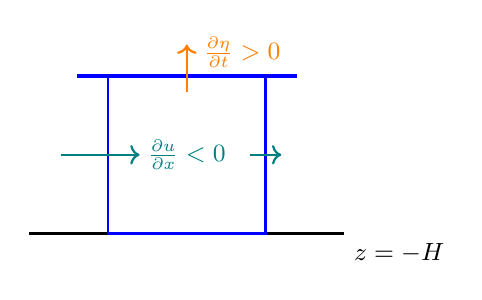
\begin{tikzpicture}[scale=2]

  % Seafloor
  \draw[very thick] (-0.5,-1) -- (1.5,-1);
  \node[below right] at (1.5,-1) {\small $z = -H$};

  % Sea surface line (extends beyond control volume)
  \draw[very thick, blue] (-0.2,0) -- (1.2,0);

  % Control volume
  \draw[thick, blue] (0,0) -- (0,-1) -- (1,-1) -- (1,0);

  % Horizontal velocity arrows
  \draw[->, thick, teal] (-0.3,-0.5) -- (0.2,-0.5); % Stronger inflow (left)
  \draw[->, thick, teal] (0.9,-0.5) -- (1.1,-0.5); % Weaker outflow (right)
  \node[teal] at (0.5,-0.5) {\small $\frac{\partial u}{\partial x} < 0$};

  % Vertical velocity at surface
  \draw[->, thick, orange] (0.5,-0.1) -- (0.5,0.2);
  \node[orange] at (0.85,0.15) {\small $\frac{\partial \eta}{\partial t}>0$};


\end{tikzpicture}

\end{document}
